\documentclass[JCDReport.tex]{subfiles} 
\begin{document}

The synchronization server propagates changes from one machine to another using a network connection. The management of the distributed VFSs is made on an account basis, i.e. in order to use the server, a user must have an account and link a virtual disk to this account. Therefore the server allows user to register and login after successful registration. Once the user enters the online mode (see GUI part) the currently open disk is synchronized to the server automatically. After initial synchronization, every synchronized disk gets a unique ID, so the disk can be identified. A user can have multiple disks, while a disk belongs to a single user. Unlinked disks are not synchronized. There is an automatic conflict recognition so the user can resolve conflicts by rolling back to a specific version, which is not conflicted, and then restart the synchronization again.\\

Technically the server is implemented as a WCF \footnote{http://msdn.microsoft.com/en-us/library/dd456779.aspx} service  and it allows multiple parallel connections. A an optional requirement, automatic persistence was implemented using SQLite. The usage of SQLite for this optional requirement was allowed by Alexey Kolesnichenko \footnote{https://piazza.com/class\#spring2013/252028400l/41}.\\

\subsection{Requirements}

% TODO: Remove this text and replace it with actual content
\emph{Describe which requirements (and possibly bonus requirements) you have implemented in this part. Give a quick description (1-2 sentences) of each requirement. List the software elements (classes and or functions) that are mainly involved in implementing each requirement.}


% 1. The browser should allow the user to create a new account or to log in to an existing account.
\subsubsection{Registration and login}
There are two forms for registration and login.\\
Classes: MainViewModel, DiskServiceClient\\
Commands: LoginCommand, LogoutCommand
\begin{figure}[h!]
	\centering
	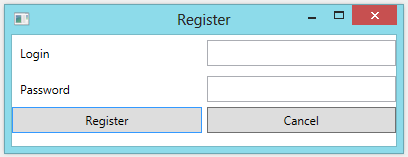
\includegraphics[scale=1]{imageslukas/registration.png}
	\caption{Registration functionality}
\end{figure}	
\begin{figure}[h!]
	\centering
	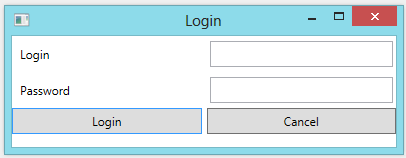
\includegraphics[scale=1]{imageslukas/login.png} 
	\caption{Login functionality}
\end{figure}	
	
% 2. The browser should offer to switch to an offine mode, and be able to operate without a connection to the server.
\subsubsection{Online / offline mode}
The user can switch between online and offline mode.\\
Classes: MainViewModel, DiskServiceClient, SynchronizationViewModel, SynchronizationService\\
Commands: SwitchToOnlineModeCommand, SwitchToOfflineModeCommand
\begin{figure}[h!]
	\centering
	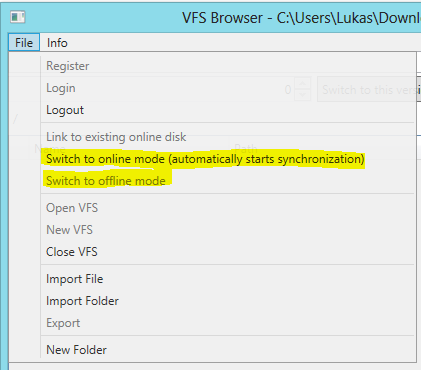
\includegraphics[scale=1]{imageslukas/onlineofflinemode.png} 
	\caption{Online and offline switch}
\end{figure}	

% 3. The browser should support binding an existing virtual disk to an active account.
\subsubsection{Binding of existing disk}
The user can bind an existing disk to the local machine. Synchronization will then start automatically.\\
Classes: MainViewModel, DiskBrowserViewModel, DiskServiceClient\\
Commands: LinkDiskCommand
\begin{figure}[h!]
	\centering
	
\includegraphics[scale=1]{imageslukas/todo.png} 
	\caption{Binding an existing virtual disk}
\end{figure}	

% 1. The server should support registration of unique accounts. Each account includes name & password.
\subsubsection{Registration of unique accounts}
The server provides a registration of unique user accounts. Each account includes name and password. To make registered users persistent, SQLite is used. If persistence would not have been implemented, a dictionary with the login as key could have been used.\\
Classes: UserDto, DiskServiceImpl, PersistenceImpl
\begin{figure}[h!]
	\centering
	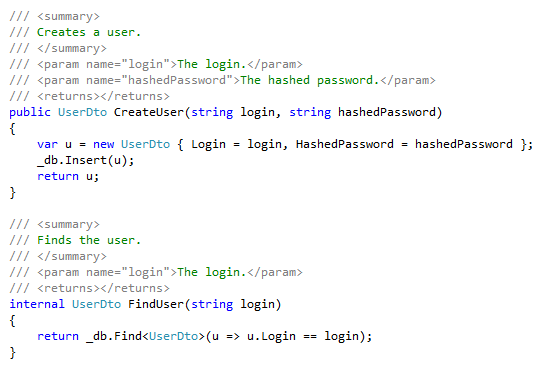
\includegraphics[scale=1]{imageslukas/login_server.png} 
	\caption{Code to persist and to find a user}
\end{figure}


% 2. The server should track changes to linked virtual disks of registered accounts and synchronize the changes across the machines.
\subsubsection{Atuomatic synchronization across machines}
Once a disk is bound to a server and the client is in online mode, the local changes are synchronized across the machines automatically. If remote changes occur, the client automatically downloads all changes from the server.
\begin{figure}[h!]
	\centering
	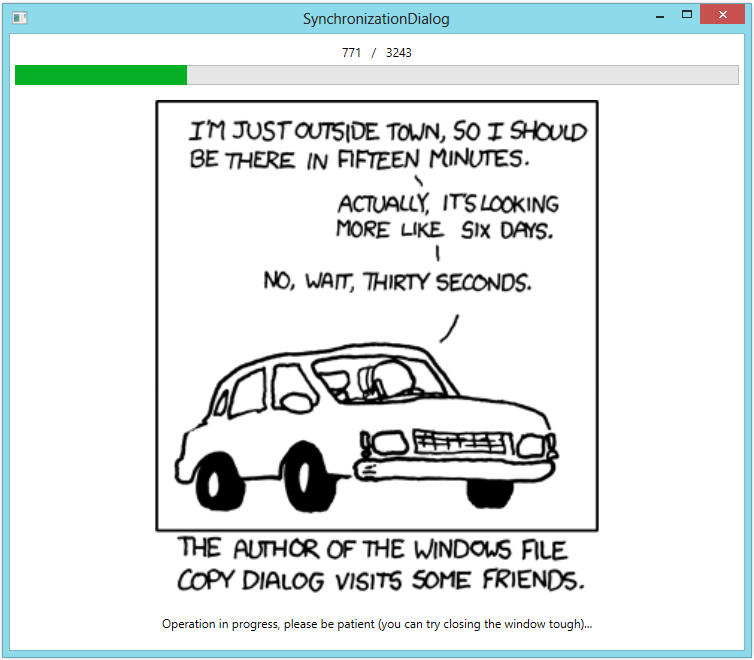
\includegraphics[scale=0.7]{imageslukas/synchronization_dialog.png} 
	\caption{The synchronization dialogue}
\end{figure}

% 1. Provide a set of mocked unit tests for your implemenation.
\subsubsection{Mocked unit tests}
Because of the IoC pattern, mocked unit tests are fairly easy to implement. For example, in the VFSConsoleTests project, the FileSystemTextManipulatorMock mocks the FileSystemTextManipulator. Therefore the console can be tested without the FileSystemTextManipulator. Additionally, there are InOutMocks to mock the input / output.
\begin{figure}[h!]
	\centering
	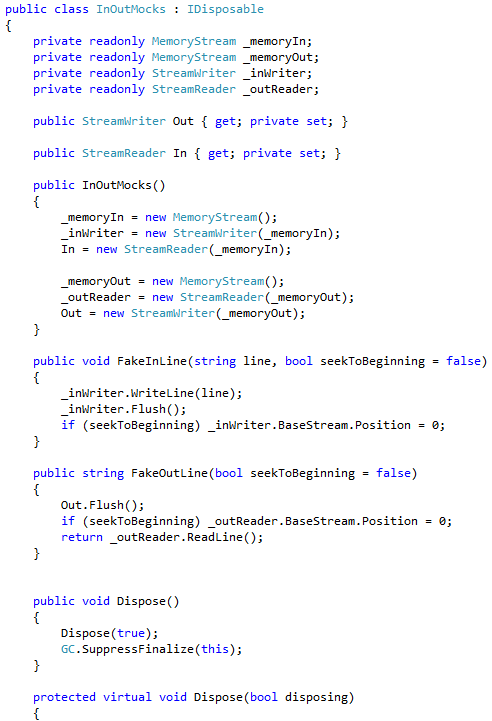
\includegraphics[scale=1]{imageslukas/inoutmocks.png} 
	\caption{The input / output mocks to test the console application}
\end{figure}

% 2. Conflict Resolution: implement a conflict resolution scheme, so that concurrent changes to the same file are not lost (e.g. saving conflicting files as separate versions).
\subsubsection{Conflict resolution}
There is an automatic conflict recognition so the user can resolve conflicts by rolling back to a specific version, which is not conflicted, and then restart the synchronization again.\\
While the file system is conflicted, read operations are still possible. This way, the user can export a file he changed, roll back to a older version, synchronize the disk, and then import the file he changed again.
\begin{figure}[h!]
	\centering
	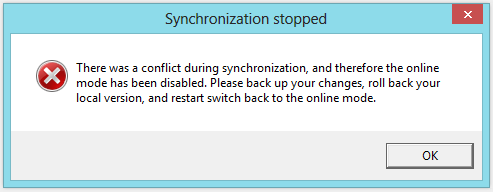
\includegraphics[scale=1]{imageslukas/synchronization_conflict1.png}
	\caption{Conflict recognition}
\end{figure}
\begin{figure}[h!]
	\centering
	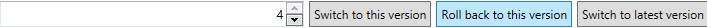
\includegraphics[scale=0.75]{imageslukas/synchronization_conflict2.png}
	\caption{Conflict resolution}
\end{figure}

% 1. The browser is updating automatically when changes to the disk occur.
\subsubsection{Automatic updates}
The browser is updating automatically when changes to the disk occur. To make this possible, the file system provides an event, which fires when changes to the file system occur. The GUI registers to this event. This is the .NET / WPF implementation which is very similar to the observer pattern.\\
Classes: FileSystem, FileSystemTextManipulator, MainViewModel\\
Events: FileSystemChanged
\begin{figure}[h!]
	\centering
	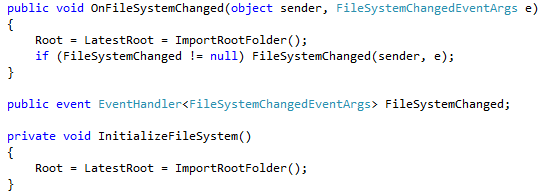
\includegraphics[scale=1]{imageslukas/file_system_changed1.png} 
	\caption{Automatic updates: the event implementation in the file system class}
\end{figure}
\begin{figure}[h!]
	\centering
	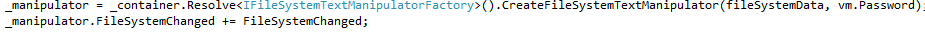
\includegraphics[scale=1]{imageslukas/file_system_changed2.png} 
	\caption{Automatic updates: the MainViewModel registers to updates when the file system is changed}
\end{figure}
\begin{figure}[h!]
	\centering
	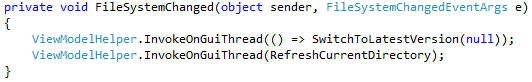
\includegraphics[scale=1]{imageslukas/file_system_changed3.png} 
	\caption{Automatic updates: Is executed when the file system is changed.}
\end{figure}


% 2. The server is able to synchronize changes, which are done simultaneously on the same account on different machines.
\subsubsection{TODO}
TODO.
\begin{figure}[h!]
	\centering
	
\includegraphics[scale=1]{imageslukas/todo.png} 
	\caption{TODO}
\end{figure}

% Incremental Changes: minimize the communication between the browser and the server by only transfering the parts of a file that changed.
\subsubsection{TODO}
TODO.
\begin{figure}[h!]
	\centering
	
\includegraphics[scale=1]{imageslukas/todo.png} 
	\caption{TODO}
\end{figure}

% 3. File History: provide a history for les and an interface to restore a previous version.
\subsubsection{TODO}
TODO.
\begin{figure}[h!]
	\centering
	
\includegraphics[scale=1]{imageslukas/todo.png} 
	\caption{TODO}
\end{figure}






% 
\subsubsection{TODO}
TODO.
\begin{figure}[h!]
	\centering
	
\includegraphics[scale=1]{imageslukas/todo.png} 
	\caption{TODO}
\end{figure}

% 
\subsubsection{TODO}
TODO.
\begin{figure}[h!]
	\centering
	
\includegraphics[scale=1]{imageslukas/todo.png} 
	\caption{TODO}
\end{figure}











\subsection{Design}

% TODO: Remove this text and replace it with actual content
\emph{Give an overview of the design of this part and describe in general terms how the implementation works. You can mention design patterns used, class diagrams, definition of custom file formats, network protocols, or anything else that helps understand the implementation.}


\subsection{Integration}

% TODO: Remove this text and replace it with actual content
\emph{If you had to change the design or API of the previous part, describe the changes and the reasons for each change here.}


\end{document}
